\documentclass{standalone}
\usepackage{tikz}
\usepackage{ctex,siunitx}
\setCJKmainfont{Noto Serif CJK SC}
\usepackage{tkz-euclide}
\usepackage{amsmath}
\usetikzlibrary{patterns, calc,3d}
\usetikzlibrary {decorations.pathmorphing,decorations.pathreplacing,decorations.shapes}
\tikzset{label style/.append style={font=\small}}
\begin{document}
\small
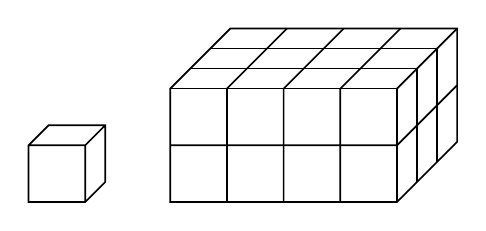
\begin{tikzpicture}[>=latex,scale=0.9,inner sep=1pt]
  \draw[semithick](0,0)--(0.8,0)--++(45:0.4)--++(0,0.8)--++(-0.8,0)--++(45:-0.4)--cycle(0.8,0)--++(0,0.8)--++(45:0.4)(0.8,0.8)--(0,0.8);
  \draw[semithick](2,0)--++(3.2,0)--++(45:1.2)--++(0,1.6)--++(-3.2,0)--++(45:-1.2)--cycle;
  \foreach \x[count=\i] in {0,0.4,0.8} 
  {
    \draw[semithick]([shift=(45:\x)]2,1.6)--++(3.2,0)--++(0,-1.6);
    \draw[semithick](2+\i*0.8,0)--++(0,1.6)--++(45:1.2);
  }
  \draw[semithick](5.2,1.6)--++(45:1.2);
  \draw[semithick](2,0.8)--(5.2,0.8)--++(45:1.2);
\end{tikzpicture}
\end{document}